\chapter{Cousins in the \fhkb}
\label{chap:cousins}
\taskstart 

In this Chapter you will
\begin{enumerate}
\item Revise or get to know about degrees and removes of cousin;
\item Add the properties and sub-property chains for first and second cousins;
\item Add properties and sub-property chains for some removes of cousins;
\item Find out that the siblings debacle haunts us still;
\item Add a defined class that does first cousins properly.
\end{enumerate}

\snapshot{There is a snapshot of the ontology as required at this point in the tutorial available at \fhkbhome.}

\dragon{Be warned; from here on the reasoner can start running slowly! Please see warning at the beginning of the last chapter for more information.}

\section{Introducing Cousins}
\label{sec:cousin_intro}

Cousins can be confusing, but here is a brief summary:
\begin{itemize}
\item First cousins share a grandparent, but are not siblings;
\item Second cousins share a great grandparent, but are not first cousins or siblings;
\item Degrees such as first and second cousin give the distance to the nearest common ancestor;
\item Removes give differences in generation. So, my Dad's first cousins (his generation) are my (\rds's) first cousins once removed.
\end{itemize}
Simply, my first cousins are my parent's sibling's children. As usual, we can think about the objects and put in place some sub-property chains.

\section{First Cousins}

Figure~\ref{fig:first_cousins} shows the sub-property chain for first cousins. As usual, think at the object level; to get to the first cousins of \rds, we go to the parents of \rds, to their siblings and then to their children. We go up, along and down. The OWL for this could be:

\owlcode{
ObjectProperty: hasFirstCousin

    SubPropertyOf: 
        hasCousin
    
    SubPropertyChain: 
        hasParent o hasSibling o hasChild
    
    Characteristics: 
        Symmetric
}

\begin{figure}
\begin{center}
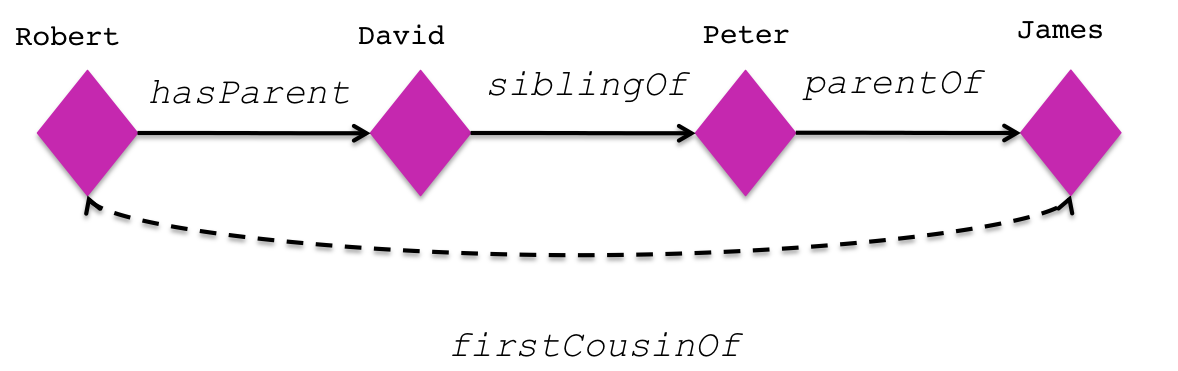
\includegraphics[width=\figwidth]{figures/cousin}
\caption{Tracing out the sub-property chain for cousins going from a child to a parent, to its sibling, and down to its child, a cousin}
\label{fig:first_cousins}
\end{center}
\end{figure}

Note that we follow the definitions in Section~\ref{sec:cousin_intro} of first cousins sharing a grandparent, but not a parent. The sub-property chain goes up to children of a grandparent (a given person's parents), along to siblings and down to their children. We do not want this property to be transitive. One's cousins are not necessarily my cousins. The blood uncles of \rds have children that are his cousins. These first cousins, however, also have a mother that is not a blood relation of \rds and the mother's sibling's children are not cousins of \rds.  

We do, however, want the property to be symmetric. One's cousins have one's-self as a cousin.

We need to place the cousin properties in the growing object property hierarchy. Cousins are obviously blood relations, but not ancestors, so they go off to one side, underneath \con{hasBloodrelation}. We should group the different removes and degree of cousin underneath one \con{hasCousin} property and this we will do.

Do the following:
\steps{First cousins}{
\item Add the property of \con{hasCousin} to the hierarchy underneath \con{hasBloodrelation};
\item Add \con{hasFirstCousin} underneath this property;
\item Add the sub-property chain as described above;
\item Run the reasoner and look at the first cousins of \rds.
}

You should see the following people as first cousins of \rds: Mark Anthony Heath, Nicholas Charles Heath, Mark Bright, Ian Bright, Janet Bright, William Bright, James Bright, Julie Bright, Clare Bright, Richard John Bright and Robert David Bright. The last two, as should be expected, are first cousins of \rds and this is not correct. As \ds will be his own brother, his children are his own nieces and nephews and thus the cousins of his own children. Our inability to infer siblings correctly in the \fhkb haunts us still and will continue to do so.

\dragon{Although the last query for the cousins of \rds should return the same results for every reasoner, we have had experiences where the results differ.}

\section{Other Degrees and Removes of Cousin}

Other degrees of cousins follow the same pattern as for first cousins; we go up, along and down. For second cousins we go up from a given individual to children of a great grandparent, along to their siblings and down to their grandchildren. The following object property declaration is for second cousins (note it uses the \con{isGrandparentOf} and its inverse properties, though the parent properties could be used) :

\owlcode{
ObjectProperty: hasSecondCousin

    SubPropertyOf: 
        hasCousin
    
    SubPropertyChain: 
        hasGrandParent o hasSibling o isGrandParentOf
    
    Characteristics: 
        Symmetric
}

`\emph{Removes}' simply add in another `leg' of either `up' or `down' either side of the `along'---that is, think of the actual individuals involved and draw a little picture of blobs and lines---then trace your finger up, along and down to work out the sub-property chain. The following object property declaration does it for first cousins once removed (note that this has been done by putting this extra `leg' on to the \con{hasFirstCousin} property; the symmetry of the property makes it work either way around so that a given person is the first cousin once removed of his/her first cousins once removed): 
\\\\
\owlcode{
ObjectProperty: hasFirstCousinOnceRemoved

    SubPropertyOf: 
        hasCousin
    
    SubPropertyChain: 
        hasFirstCousin o hasChild
    
    Characteristics: 
        Symmetric
}
\\\\
To exercise the cousin properties do the following:
\steps{Cousin properties}{
\item Add properties for second degree cousins;
\item Add removes for first and second degree cousins;
\item Run the reasoner and check what we know about \rds' other types of cousin.
}
You should see that we see some peculiar inferences about \rds' cousins -- not only are his brother and himself his own cousins, but so are his father, mother, uncles and so on. This makes sense if we look at the general sibling problem, but also it helps to just trace the paths around. If we go up from one of \rds' true first cousins to a grandparent and down one parent relationship, we follow the first cousin once removed path and get to one of \rds' parents or uncles. This is not to be expected and we need a tighter definition that goes beyond sub-property chains so that we can exclude some implications from the \fhkb.
%\todo{check and finish}

\section{Doing First Cousins Properly}

As far as inferring first cousin facts for \rds, we have failed. More precisely, we have recalled all \rds's cousins, but the precision is not what we would desire. What we can do is ask for \rds' cousins, but then remove the children of \rds' parents. The following DL query achieves this:

\owlcode{
Person that hasFirstCousin value \irds 

and (not (hasFather value \ids) or not (hasMother value \imgs)
}
\\
This works, but only for a named individual. We could make a defined class for this query; we could also make a defined class \con{FirstCousin}, but it is not of much utility. We would have to make sure that people whose parents are not known to have siblings with children are excluded. That is, people are not `first cousins' whose only first cousins are themselves and their siblings. The following class does this:

\owlcode{
Class: FirstCousin

EquivalentTo: Person
	that hasFirstCousin some Person
}

\steps{Roberts first cousins}{
\item Make a defined class \con{FirstCousin} as shown above;
\item Make a defined class \con{FirstCousinOfRobert};
\item Create a DL query that looks at \irds first cousins and takes away the children of \irds' parents as shown above.
}
This gives some practice with negation. One is making a class and then `taking' some of it away -- `these, but not those'.\herebedragons 
%\todo{perhaps a bit ore about negation?}

\section{Summary}

We have now expanded the \fhkb to include most blood relationships. We have also found that cousins are hard to capture just using object properties and sub-property chains. Our broken sibling inferences mean that we have too many cousins inferred at the instance level. We can get cousins right at the class level by using our inference based cousins, then excluding some using negation. Perhaps not neat, but it works.

We have reinforced that we can just add more and more relationships to individuals by just adding more properties to our \fhkb object property hierarchy and adding more sub-property chains that use the object properties we have built up upon parentage and sibling properties; this is as it should be.
\\

\expressivity{SROIQ(D)}

\ctime{0}{111395}{868}